\documentclass[t,14pt]{beamer}
\setbeamersize{text margin left=8mm,text margin right=8mm}

\usepackage{xeCJK}
\setCJKmainfont{Noto Sans CJK SC}
\setCJKmonofont{Noto Sans Mono CJK SC}
\setCJKsansfont{Noto Sans CJK SC}
\CJKsetecglue{}

\usetheme[sectionpage=none,block=fill]{metropolis}
\usepackage{appendixnumberbeamer}

\usepackage{booktabs}
\usepackage[scale=2]{ccicons}

\usepackage{graphicx}
\usepackage{subcaption}
\captionsetup[subfigure]{subrefformat=simple,labelformat=simple}
\renewcommand\thesubfigure{(\alph{subfigure})}
\usepackage{caption}
\captionsetup[table]{skip=0mm}
\usepackage{float}
\usepackage{adjustbox}

\usepackage{enumerate}
\setlength{\leftmargini}{5pt}
\setlength{\leftmarginii}{8pt}
\setbeamertemplate{itemize item}[square]
\setbeamertemplate{itemize subitem}[circle]
\setbeamertemplate{itemize subsubitem}[triangle]

\usepackage[backend=biber,citestyle=numeric-comp,sorting=none]{biblatex}
\addbibresource{main.bib}
\renewcommand*{\bibfont}{\scriptsize}

\usepackage{amsmath}
\usepackage{amsfonts}
\usepackage{amssymb}
\usepackage{bm}

\usepackage{array}
\usepackage{tabularx}
\usepackage{multirow}
\usepackage{calc}


\newenvironment{lead}{
  \vspace*{8pt}
  \begin{beamercolorbox}[wd=\dimexpr\linewidth+20pt\relax,sep=8pt,shadow=false,rounded=false]{block body example}
}{
  \end{beamercolorbox}
}


\title{Deriving Machine Attention from Human Rationales}
%\subtitle{beamerテンプレート}
\author{@koreyou}
\date[]{2018/12/9}
\institute{EMNLP2018読み会@サイバーエージェント, 東京}
%\titlegraphic{\includegraphics[scale=0.3]{logo.png}}

% subject and keywords are embedded as PDF meta info
%\subject{}
\keywords{論文読み,自然言語処理,深層学習,機械学習}

\begin{document}

\frame{\titlepage}

\begin{frame}{Who am I?}
  \begin{columns}[onlytextwidth]
  \begin{column}{0.68\linewidth}
    \begin{itemize}
      \item 是枝祐太
      \item 某電機会社リサーチャー
      \item 研究歴
      \begin{itemize}
        \item 〜2015: 医療+ロボット(大学)
        \item 〜2016: ロボット+応用機械学習
        \item 〜現在: \alert{応用機械学習+自然言語処理}
      \end{itemize}
    \end{itemize}
  \end{column}
  \begin{column}{0.3\linewidth}
    \begin{itemize}
      \item[] \raisebox{-0.3\height}{
\includegraphics[width=6mm]{fig/GitHub-Mark-64px.png}} koreyou
      \item[] \raisebox{-0.3\height}{
\includegraphics[width=6mm]{fig/Twitter_Social_Icon_Square_Color.png}} koreyou\_
    \end{itemize}
    \vspace*{10mm}
    \only<1>{\adjincludegraphics[width=0.95\linewidth,valign=t]{fig/my_weight_1.png}}
    \only<2>{\adjincludegraphics[width=0.95\linewidth,valign=t]{fig/my_weight_2.png}}
  \end{column}
  \end{columns}
\end{frame}

\begin{frame}{tl;dr}
% TODO: write tl;dr
\end{frame}

\begin{frame}{Table of contents}
  \setbeamertemplate{section in toc}[sections numbered]
  \tableofcontents[hideallsubsections]
\end{frame}

\begin{frame}[c]
  \begin{center}
    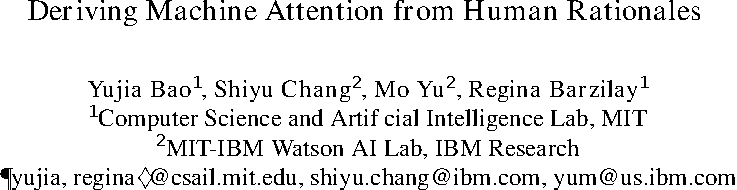
\includegraphics[width=\linewidth]{fig/title.pdf}    
  \end{center}
\end{frame}

\section{背景}
\frame[standout]{\insertsection}

\begin{frame}{観点付き評判分析}
\begin{lead}
    リード文
\end{lead}
\begin{itemize}
\item 本研究は自然言語タスク全般に利用可能
\begin{itemize}
    \item わかりやすさのために具体的なタスクを先に紹介
\end{itemize}
\item 観点付き評判分析 (Aspect-based sentiment analysis; ABSA)
\begin{itemize}
    \item 入力文が各観点について肯定的か否定的かを分類
\end{itemize}
\end{itemize}
\end{frame}

\begin{frame}{Rationale (根拠、解釈)}
\begin{lead}
    根拠 (Rationale) 提示型AIが注目されている
\end{lead}
\begin{itemize}
\item 分類の\alert{根拠}となる記載箇所
\begin{itemize}
    \item なぜその予測をしたかの\alert{解釈}を与えAIを\alert{説明可能}にする
\end{itemize}
\item Rationaleを提示する研究が注目されている\cite{lei_2016,ling_2017}
\end{itemize}
\end{frame}

\begin{frame}{研究目的}
\begin{lead}
    根拠データを使い低リソースドメインで精度向上
\end{lead}
\begin{itemize}
\item 分類の教師データに加え、なぜそのような分類をすべきかという\alert{根拠を学習に加える}ことで、\alert{少量のデータで高い分類精度}を実現できないか?
\end{itemize}
\end{frame}

\begin{frame}{文分類におけるAttention機構の活用}
\begin{lead}
    Attention機構により文分類の精度向上が図れる
\end{lead}
\begin{itemize}
\item プーリングとしてのattention機構
\begin{itemize}
    \item 各単語表現からattentionの値 (実数) を計算
    \item attentionの値で単語表現の重み付き和
\end{itemize}
\end{itemize}

\vspace*{-8pt}
\begin{figure}[H]
  \centering
  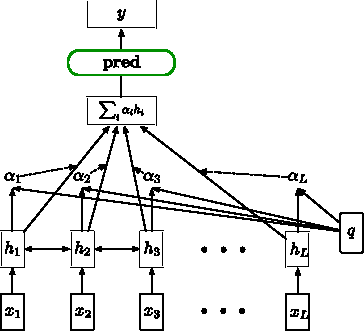
\includegraphics[width=40mm]{fig/attention_classifier.pdf}
  \caption{文分類におけるAttention機構\cite{bao_2018}}
\end{figure}
\end{frame}

\begin{frame}{Attention vs. Rationale}
\begin{lead}
    RationaleをAttention風に変換する
\end{lead}
\begin{itemize}
\item Attention $\neq$ Rationale
\begin{itemize}
    \item Attentionは連続値(強弱がある)、rationaleは二値
    \item Attentionは分類精度を最大化するよう最適化されている
\end{itemize}
\item Rationaleを学習に使うよりも、Rationaleをattention\textbf{風}に変換してから学習に使うほうが良いのでは?
\begin{itemize}
    \item 分類の学習に望ましいAttentionを\alert{真(oracle) attention}と呼ぶ
\end{itemize}
\end{itemize}
\end{frame}

\begin{frame}{Attention}
\begin{lead}
    RationaleをAttention風に変換する
\end{lead}
\begin{itemize}
\item Oracle attentionは大量の正解分類データを用い分類を学習することで獲得できる
\item 正解分類データが少ないドメインではRationale$\Rightarrow$真attentionの変換は学習できない
\item データが多いドメインでの変換を転移
\end{itemize}
\begin{exampleblock}{仮説}
Rationale$\Rightarrow$真attentionはドメインによらず共通
\end{exampleblock}
\end{frame}


\begin{frame}[c]

  Get the presentation slides from:

  \begin{center}blah blah\end{center}

  This presentation is licensed under
    \href{https://creativecommons.org/publicdomain/zero/1.0/}{
    CC0 1.0 Universal (CC0 1.0) Public Domain Dedication}.

  \begin{center}\cczero\end{center}

\end{frame}

\begin{frame}[allowframebreaks]{References}
  \printbibliography[heading=none]
\end{frame}

\end{document}

